\section{Understanding the eUTxO Model and Its Components} \label{sec:exploring}

Two popular record-keeping models in blockchain networks are the eUTXO (Extended Unspent Transaction Output) Model used by Cardano and the Account/Balance Model employed by Ethereum. This section provides a basic understanding of these models, their differences, and their respective pros and cons.

\section{eUTXO Model}
In Cardano, each transaction spends outputs from prior transactions and generates new outputs for future transactions. All unspent transactions are stored in each fully synchronized node, giving rise to the name ``eUTXO''. A user’s wallet tracks unspent transactions associated with the user's addresses, and the wallet balance is the sum of these unspent transactions.

\subsection{Example}
1. Alice gains 12.5 ADA through staking rewards, resulting in one eUTXO of 12.5 ADA.

2. Alice sends 1 ADA to Bob. Alice’s wallet uses her eUTXO of 12.5 ADA, sending 1 ADA to Bob and receiving 11.5 ADA as a new eUTXO to a new address owned by Alice.

3. If Bob had an eUTXO of 2 ADA before step 2, his wallet now shows a balance of 3 ADA from two eUTXOs.

\subsection{Account/Balance Model}
The Account/Balance Model maintains the balance of each account as a global state. It checks that an account's balance is sufficient to cover the transaction amount.

\subsection{Example}
1. Alice gains 5 ETH through mining, recorded in the system.

2. Alice sends 1 ETH to Bob, reducing her balance to 4 ETH.

3. Bob’s balance increases by 1 ETH, so if he had 2 ETH initially, he now has 3 ETH.

\subsection{Analogies}
\begin{itemize}
    \item  \textbf{eUTXO Model}: Similar to using paper bills, where each bill (eUTXO) can be spent once, and change is returned as new eUTXOs.
    \item \textbf{Account/Balance Model}: Similar to a bank's ATM/debit card system, where the bank ensures sufficient balance before approving transactions.
\end{itemize}

\subsection{Benefits}

\subsection{eUTXO Model}
\begin{itemize}
    \item \textbf{Scalability}: Enables parallel transactions and scalability innovations.
    \item \textbf{Privacy}: Provides higher privacy, especially with new addresses for each transaction.
\end{itemize}

\subsection{Account/Balance Model}
\begin{itemize}
    \item \textbf{Simplicity}: Easier for developers of complex smart contracts requiring state information.
    \item \textbf{Efficiency}: More efficient as each transaction only validates account balance.
\end{itemize}

\subsection*{Drawbacks}
\textbf{Account/Balance Model}: Susceptible to double-spending attacks, counteracted by an incrementing nonce.

Both models have trade-offs and are chosen based on specific blockchain needs. Some blockchains, like Hyperledger, adopt eUTXO to benefit from Bitcoin's innovations.


\section{Writing Transactions and Validating Inputs and Outputs}

In this section, we'll analyze the components of a Cardano transaction and how it is built using a Cardano node and then using the Lucid library.

Let's start with the following transaction:

\href{https://preview.cexplorer.io/tx/a2fcdf32987ebb729ab8f63b377e360ececbf4805713ff559d2b69bb3c543a01}{a2fcdf32987ebb729ab8f63b377e360ececbf4805713ff559d2b69bb3c543a01}

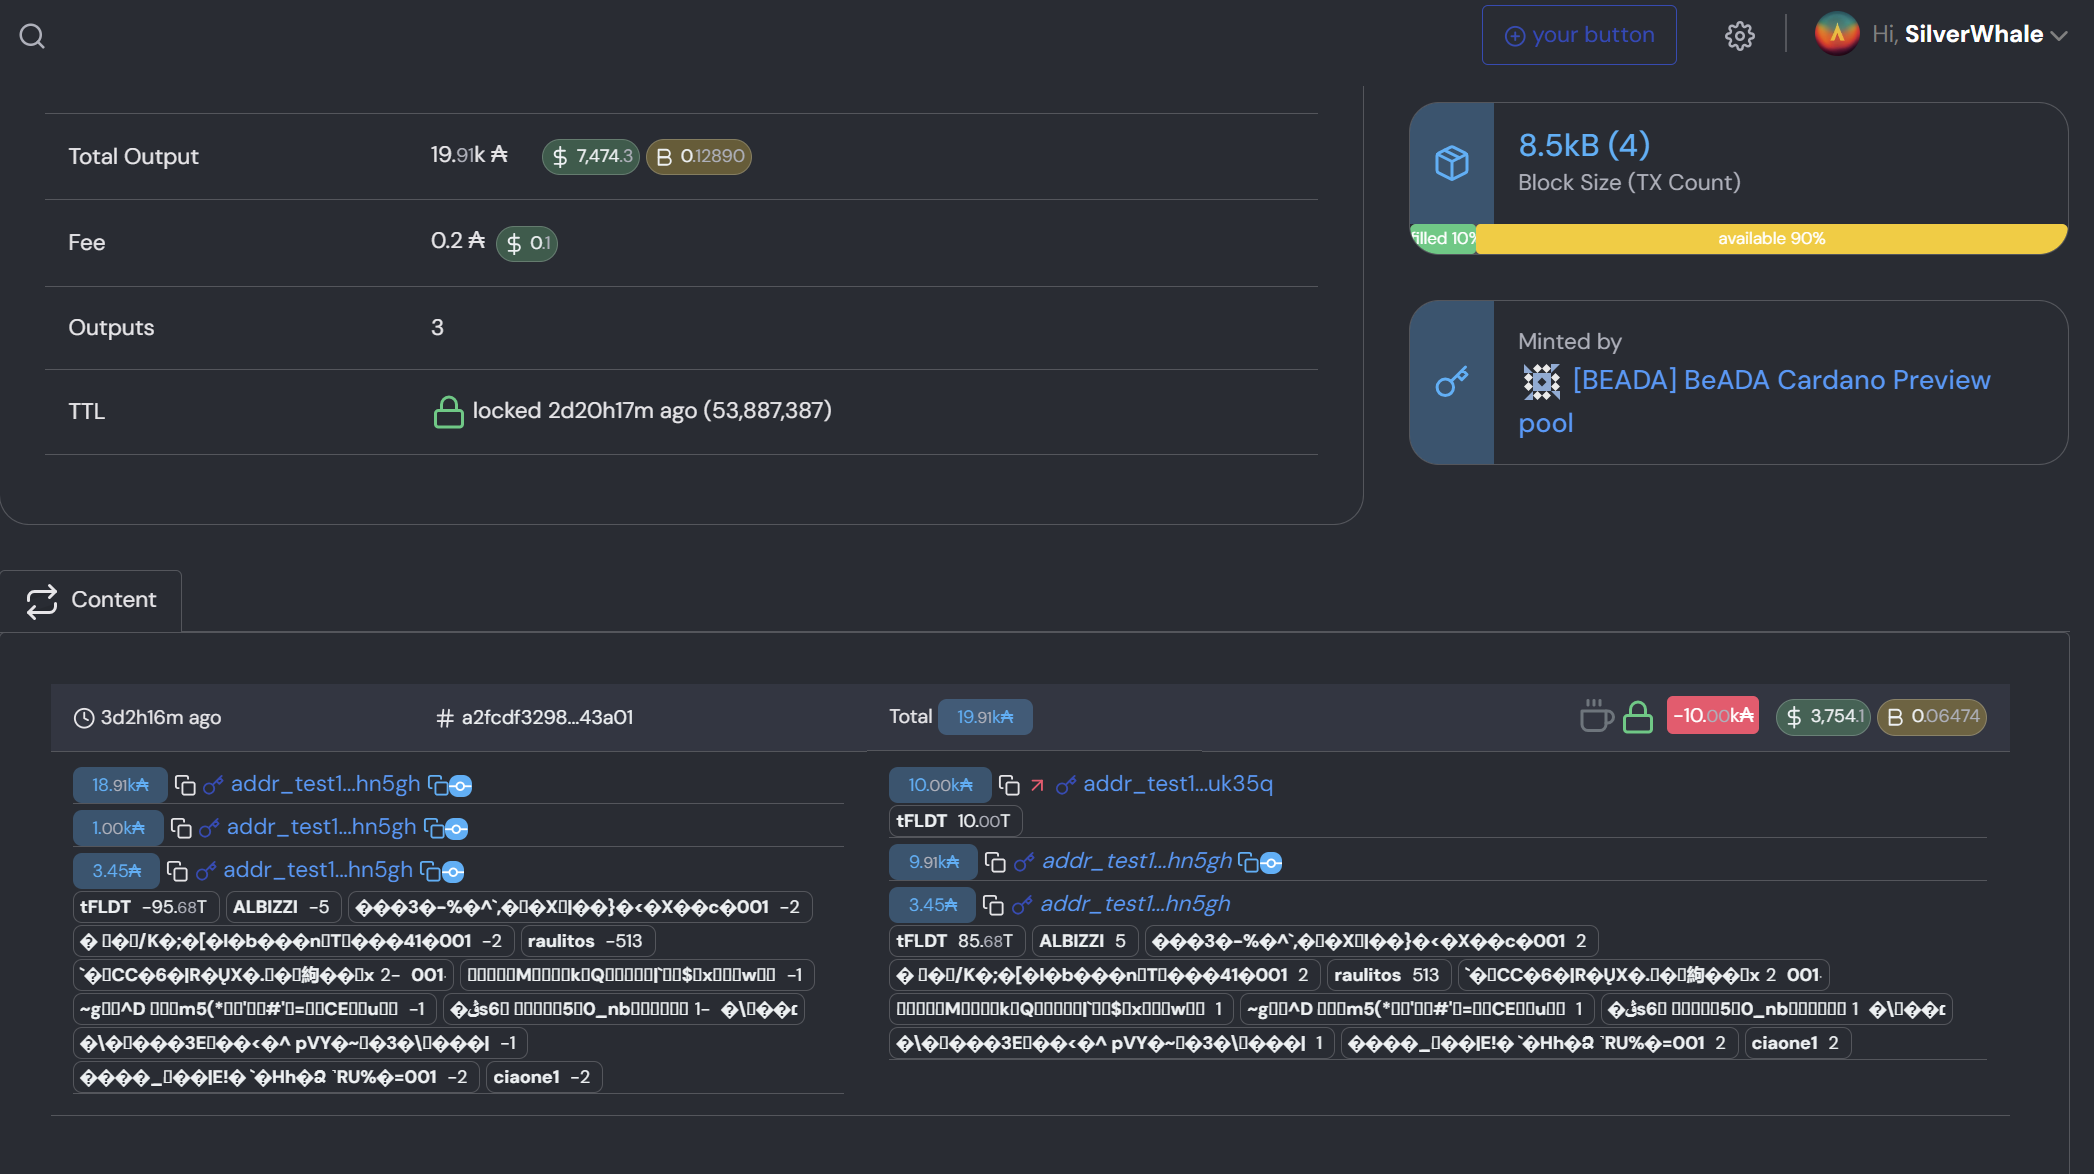
\includegraphics[scale=0.3]{transactionTestnet}

Let's analyze what we can see here:

On the \textbf{left}, we have the \gls{inputs} of the transaction. We can see that we are spending 3 inputs containing tADA and some tokens.
The inputs being spent are from the following transactions:

\begin{itemize}
    \item \texttt{5df4a4fb78650b5d8b0e761e0ade2c2ab2289b4feb97f6780b82d78b3d02bf70}
    \item \texttt{f0e29aed793164ce8192aec7ec647b7e7747206d701b0dfd4a810414f7acb96b}
    \item \texttt{5df4a4fb78650b5d8b0e761e0ade2c2ab2289b4feb97f6780b82d78b3d02bf70}
\end{itemize}

This means that for each transaction, we can obtain the transactions that generated the funds being spent directly from the hash of the inputs.
Not just this, it means that we are always able to track if the funds generated by a transaction have already been spent because they will appear as input on another transaction.

But that's not all; for each input, we are able to see from which address they come from, in this case \texttt{addr\_test1qqw...hn5gh} and also the amount of tADA and tokens that were locked inside those inputs. We'll call this \textbf{Value}.

On the \textbf{right} side, we can see the outputs of the transaction. Therefore, where is the tADA going?

We have 3 outputs:

\begin{itemize}
    \item The first output is sending 10,000 tADA and 1M tFLDT to \texttt{addr\_test1qpku...sjuk35q}.
    \item The second output is a change to \texttt{addr\_test1qqwywxe3ag9sf3jjhk8hd...fhn5gh} sending back all the tADA that was left.
    \item The third output is a change to \texttt{addr\_test1qqwywxe3ag9sf3jjhk8hd...fhn5gh} sending back all the NFTs and tokens that were leftovers.
\end{itemize}

Finally, we can see that this transaction was validated during \gls{epoch} 623, \gls{block} 2,270,567, and \gls{slot} 53,865,862.
It was confirmed by BEADA stake pool operator, and there was a 0.2 fee paid to the network.

\subsection{Build a transaction with Cardano node}

This part is not mandatory since it requires to run a Cardano node, however it is interesting to see how a transaction is built from scretch


Let's create a folder:

\begin{lstlisting}
mkdir exercise01
\end{lstlisting}

Now we create the wallet with:

\begin{lstlisting}
cardano-cli address key-gen --verification-key-file payment.vkey --signing-key-file payment.skey
\end{lstlisting}

To see the address, use the following command:

\begin{lstlisting}
cardano-cli address build --payment-verification-key-file payment.vkey --out-file payment.addr
\end{lstlisting}

And then:

\begin{lstlisting}
cat payment.addr
\end{lstlisting}

And we now see our address!

\subsection*{Checking funds in wallet}

Let's run the command:

\begin{lstlisting}
cardano-cli query utxo --address $(cat payment.addr) --mainnet
\end{lstlisting}

We will see that there are no transactions, so 0 ADA.

\subsection*{Sending funds}

Let's send some ADA to the wallet from our main wallet (try with 5 ADA) and run the command again to check the transactions:

\begin{lstlisting}
cardano-cli query utxo --address $(cat payment.addr) --mainnet
\end{lstlisting}

Now we should see some ADA. For instance, 5,000,000 lovelace means 5 ADA.

\subsection*{Check funds of any address}

If you want to check the ADA inside any wallet, the command becomes:

\begin{lstlisting}
cardano-cli query utxo --address ADDRESSTOCHECKHERE --mainnet
\end{lstlisting}

The result is all the transactions containing ADA and NFTs in the address.

\subsection*{Creating the raw transaction}

Let's copy the transaction hash that contains the 5 ADA and the index:

\begin{lstlisting}
cardano-cli transaction build-raw --fee 0 --tx-in HASHOFUNSPENTTRANSACTION#INDEX --tx-out ADDRESSRECEIVER+2000000 --tx-out $(cat payment.addr)+0 --mainnet --out-file matx.raw
\end{lstlisting}

\subsection*{Calculate the fee}

We must calculate the fee according to the network parameters that we get with the following:

\begin{lstlisting}
cardano-cli query protocol-parameters --mainnet --out-file protocol.json
\end{lstlisting}

Now:

\begin{lstlisting}
cardano-cli transaction calculate-min-fee --tx-body-file matx.raw --tx-in-count 1 --tx-out-count 2 --witness-count 1 --mainnet --protocol-params-file protocol.json
\end{lstlisting}

And we get the fee we should pay at least.

\subsection*{Build the final transaction}

Now we can finally build the complete transaction with:

\begin{lstlisting}
cardano-cli transaction build-raw --fee FEE_WE_CALCULATED --tx-in HASHOFUNSPENTTRANSACTION#INDEX --tx-out ADDRESSRECEIVER+2000000 --tx-out $(cat payment.addr)+BALANCE_MINUS_FEES_MINUS_2_ADA --mainnet --out-file matx.raw
\end{lstlisting}

At this point, the transaction is finished. We must sign it with the key to prove we are the owners.

\subsection*{Signing the transaction and submitting it to the blockchain}

\begin{lstlisting}
cardano-cli transaction sign --signing-key-file payment.skey --mainnet --tx-body-file matx.raw --out-file matx.signed
\end{lstlisting}

Now using the key in the folder, we approved the transactions, we can send it to the blockchain.

\subsection*{Submitting the transaction}

To send it to the blockchain, we can launch the following:

\begin{lstlisting}
cardano-cli transaction submit --tx-file matx.signed
\end{lstlisting}

And now, after it has been processed, our balance will decrease.

\subsection{Building a Transaction with Lucid}

The \textit{Lucid} library was the very first library to accelerate development on Cardano. The main advantage of this library is its capability to make the entire process faster and easier. The previous example can be simplified as follows:

\begin{lstlisting}
const tx = await lucid.newTx()
  .payToAddress("ADDRESSRECEIVER", {lovelace: 2000000n})
  .complete();
const signedTx = await tx.sign().complete();
const txHash = await signedTx.submit();
\end{lstlisting}

There is no doubt why \textit{Lucid} has been used by the majority of the \textbf{dApps} developed on Cardano.

\section{Cardano Native Scripts}

Cardano introduced \textit{native scripts} as a foundational feature in the Shelley era, which predated the advent of smart contracts. These scripts provide a way to define complex conditions for spending funds, extending the functionality available in Bitcoin through its script language. While Bitcoin scripts include features like \textit{multisignature} and \textit{timelock}, Cardano's native scripts build upon these concepts with more sophisticated capabilities.

This section explores Cardano's native scripts, focusing on \textit{multisignature scripts} and \textit{time locking}, and comparing them to Bitcoin scripts. 

\subsection{Comparison with Bitcoin Scripts}

Bitcoin scripts are a simple stack-based language primarily used for two main features:
\begin{itemize}
    \item \textbf{Multisignature}: Requires multiple signatures to authorize a transaction. For example, a 2-of-3 multisignature scheme requires any two of three possible signatures.
    \item \textbf{Timelock}: Restricts spending of funds until a certain time or block height. Examples include \textit{CheckLockTimeVerify} which locks funds until a specific block height or timestamp.
\end{itemize}

Cardano extends these features with more advanced scripting capabilities in its native script language.


In the Shelley era and beyond, Cardano introduced a more expressive scripting language that includes \textit{multisignature scripts}. These scripts are used to create addresses that require multiple cryptographic signatures to authorize transactions. 

\subsection{Description}

A multisignature script address is one where a transaction must meet specific conditions, such as collecting signatures from multiple keys. The script defines these conditions, and the transaction witness includes both the script and the required signatures.

\subsection{Multisig Script Language}

The multisig script language uses a simple expression tree with four primary constructors:

\begin{itemize}
    \item \textbf{RequireSignature}: \texttt{RequireSignature vkeyhash} - Validates that a transaction includes a signature corresponding to the given verification key hash.
    \item \textbf{RequireAllOf}: \texttt{RequireAllOf <script> *} - Requires that all included scripts are satisfied.
    \item \textbf{RequireAnyOf}: \texttt{RequireAnyOf <script> *} - Requires that at least one of the included scripts is satisfied.
    \item \textbf{RequireMOf}: \texttt{RequireMOf <num> <script> *} - Requires that at least M of the included scripts are satisfied.
\end{itemize}

\subsection{JSON Script Syntax}

Multisignature scripts can be represented in JSON as follows:

\begin{lstlisting}
{
  "type": "sig",
  "keyHash": "e09d36c79dec9bd1b3d9e152247701cd0bb860b5ebfd1de8abb6735a"
}
\end{lstlisting}

KeyHash is the publicKey of the address allowed to spend from this multisignature, in this case is a simple 1 of 1 multisignature script.

\subsection{Time Locking Scripts}

Cardano introduced time-locking features to the native script language. This extension enables the creation of scripts that restrict transactions based on time conditions.

\subsection{Description}

Time-locking allows conditions like:

\begin{itemize}
    \item \textbf{RequireTimeBefore}: The current slot number must be before a specified slot.
    \item \textbf{RequireTimeAfter}: The current slot number must be after a specified slot.
\end{itemize}

\subsection{JSON Script Syntax}

Time-locking scripts can be represented in JSON as follows:

\begin{lstlisting}
{
  "type": "all",
  "scripts":
  [
    {
      "type": "after",
      "slot": 1000
    },
    {
      "type": "sig",
      "keyHash": "966e394a544f242081e41d1965137b1bb412ac230d40ed5407821c37"
    }
  ]
}
\end{lstlisting}

This example shows a script where there are two rules, only the owner of this publicKey can use it: 966e394a544f242081e41d1965137b1bb412ac230d40ed5407821c37 
and additionally only after the slot 1000.


\subsection{Multisignature Script Example}

\textbf{Step 1: Create a Multisignature Script Address}

\begin{lstlisting}
{
  "type": "all",
  "scripts":
  [
    {
      "type": "sig",
      "keyHash": "e09d36c79dec9bd1b3d9e152247701cd0bb860b5ebfd1de8abb6735a"
    },
    {
      "type": "sig",
      "keyHash": "a687dcc24e00dd3caafbeb5e68f97ca8ef269cb6fe971345eb951756"
    },
    {
      "type": "sig",
      "keyHash": "0bd1d702b2e6188fe0857a6dc7ffb0675229bab58c86638ffa87ed6d"
    }
  ]
}
\end{lstlisting}

This type of multisig is a 3 of 3 multisignature, all the 3 signatures must approve the spending of the funds from the address

\textbf{Step 2: Create the Address}

\begin{verbatim}
cardano-cli address \
  --payment-script-file allMultiSigScript.json \
  --testnet-magic 42 \
  --out-file script.addr
\end{verbatim}

\textbf{Step 3: Construct and Submit a Transaction}

\begin{verbatim}
cardano-cli transaction build-raw \
    --invalid-hereafter 1000 \
    --fee 0 \
    --tx-in <utxoinput> \
    --tx-out "$(cat script.addr) <amount>" \
    --out-file txbody

cardano-cli transaction witness \
  --tx-body-file txbody \
  --signing-key-file <utxoSignKey> \
  --testnet-magic 42 \
  --out-file utxoWitness

cardano-cli transaction assemble \
  --tx-body-file txbody \
  --witness-file utxoWitness \
  --out-file allWitnessesTx
\end{verbatim}

\textbf{Step 4: Submit the Transaction}

\begin{verbatim}
cardano-cli transaction submit \
  --tx-file allWitnessesTx \
  --testnet-magic 42
\end{verbatim}

\subsection{Time Locking Script Example}

\textbf{Example JSON for a Time Locking Script}

\begin{lstlisting}
{
  "type": "all",
  "scripts":
  [
    {
      "type": "after",
      "slot": 1000
    },
    {
      "type": "sig",
      "keyHash": "966e394a544f242081e41d1965137b1bb412ac230d40ed5407821c37"
    }
  ]
}
\end{lstlisting}

\textbf{Step 1: Create the Address}

\begin{verbatim}
cardano-cli address \
  --payment-script-file timeLockScript.json \
  --testnet-magic 42 \
  --out-file script.addr
\end{verbatim}

\textbf{Step 2: Construct and Submit a Transaction}

\begin{verbatim}
cardano-cli transaction build-raw \
    --invalid-before 1000 \
    --fee 0 \
    --tx-in <txin of script address> \
    --tx-out <yourspecifiedtxout> \
    --out-file spendScriptTxBody

cardano-cli transaction witness \
  --tx-body-file spendScriptTxBody \
  --script-file timeLockScript.json \
  --testnet-magic 42 \
  --out-file scriptWitness

cardano-cli transaction witness \
  --tx-body-file spendScriptTxBody \
  --signing-key-file <paySignKey> \
  --testnet-magic 42 \
  --out-file keyWitness

cardano-cli transaction assemble \
  --tx-body-file spendScriptTxBody \
  --witness-file scriptWitness \
  --witness-file keyWitness \
  --out-file spendTimeLockTx
\end{verbatim}

\textbf{Step 3: Submit the Transaction}

\begin{verbatim}
cardano-cli transaction submit \
  --tx-file spendTimeLockTx \
  --testnet-magic 42
\end{verbatim}

\section{Using Lucid Library for Cardano Native Scripts}

Working with Cardano native scripts can be made significantly easier and faster by using the Lucid library in JavaScript. This library simplifies many operations that would otherwise require complex command-line interactions. Here, we'll demonstrate how to import a Cardano native script and perform transactions using the Lucid library.

\subsection{Importing and Using Lucid Library}

The Lucid library provides a user-friendly interface for interacting with Cardano, allowing developers to perform tasks quickly and efficiently. Here’s an example of how to import a Cardano native script and use it for transactions.

\subsubsection{Example: Importing a Native Script and Performing a Transaction}

First, we need to import the necessary modules from the Lucid library:

\begin{lstlisting}
import { Lucid, Blockfrost, Constr, Utils } from "https://unpkg.com/lucid-cardano@0.9.6/web/mod.js";
\end{lstlisting}

Next, initialize the Lucid library with Blockfrost and specify the network:

\begin{lstlisting}
const lucid = await Lucid.new(
new Blockfrost("https://cardano-mainnet.blockfrost.io/api/v0", "APIKEYHERE"),
"Mainnet",
);
\end{lstlisting}

Now, we can define a multisignature script in JSON format and convert it to a native script using Lucid:

\begin{lstlisting}
const multisigScript = lucid.utils.nativeScriptFromJson(
{
"type": "all",
scripts: [
{ type: "sig", keyHash: "1c471b31ea0b04c652bd8f76b239aea5f57139bdc5a2b28ab1e69175" },
],
}
);
\end{lstlisting}

With the multisignature script, we can create the corresponding address:

\begin{lstlisting}
const multisigAddress = lucid.utils.validatorToAddress(multisigScript);
\end{lstlisting}

Finally, we can construct, sign, and submit a transaction:

\begin{lstlisting}
var tx = await lucid
.newTx()
.payToAddress(multisigAddress, { lovelace: 1000000 }) // Example: sending 1 ADA
.attachMintingPolicy(multisigScript)
.addSignerKey("1c471b31ea0b04c652bd8f76b239aea5f57139bdc5a2b28ab1e69175") // Signer key
.complete();

const signedTx = await tx.sign().complete();
const txHash = await signedTx.submit();
console.log(txHash);
\end{lstlisting}

\subsection{Advantages of Using Lucid Library}

Using the Lucid library for managing Cardano native scripts offers several advantages over traditional command-line methods:

\begin{itemize}
\item \textbf{Ease of Use}: The Lucid library abstracts away much of the complexity involved in script and transaction management, making it easier for developers to interact with the Cardano blockchain.
\item \textbf{Speed}: Transactions and script operations can be performed more quickly without the need to manually handle and submit command-line operations.
\item \textbf{Flexibility}: JavaScript provides a more flexible environment for developing and testing blockchain interactions compared to the command-line interface.
\item \textbf{Integration}: Lucid can be easily integrated into web applications and other JavaScript-based projects, facilitating broader use cases and seamless user experiences.
\end{itemize}

\section{Interacting with Smart Contracts Using Lucid}

In this section we'll see how a transaction including smart contracts on Cardano is done, don't worry if you don't get most of it. Focus on looking at the similarities with using a cardano native script as shown before.

Interacting with smart contracts on the Cardano blockchain using the Lucid library is straightforward and similar to working with native scripts, such as multisignature scripts. However, smart contracts introduce more complex logic, enabling advanced functionalities. In this section, we'll demonstrate how to use a minting smart contract to create tokens on Cardano using Lucid.

\subsection{Minting Tokens with a Smart Contract}

The process of interacting with a smart contract involves defining the contract's logic and using it in a transaction. The example below illustrates how to mint tokens using a smart contract, showcasing how similar the code structure is to working with native scripts while allowing for more sophisticated operations.

\subsubsection{Example: Using a Minting Smart Contract}

First, we need to import the necessary modules from the Lucid library and initialize it with Blockfrost:

\begin{lstlisting}
import { Lucid, Blockfrost, toHex, fromHex, Data, Constr, fromText } from "https://unpkg.com/lucid-cardano@0.10.0/web/mod.js";

const lucid = await Lucid.new(
new Blockfrost("https://cardano-mainnet.blockfrost.io/api/v0", "APIKEYHERE"),
"Mainnet",
);
\end{lstlisting}

Next, import the Plutus script data and encode it using CBOR:

\begin{lstlisting}
import data from '/plutus.json' assert { type: "json" };
console.log(data);

import * as cbor from "https://deno.land/x/cbor@v1.4.1/index.js";

const mintingPolicy = {
type: "PlutusV2",
script: toHex(cbor.encode(fromHex(data.validators[1].compiledCode)))
};

const storageScript = {
type: "PlutusV2",
script: toHex(cbor.encode(fromHex(data.validators[0].compiledCode)))
};
\end{lstlisting}

Enable the Nami wallet and select it with Lucid:

\begin{lstlisting}
const api = await window.cardano.nami.enable();
lucid.selectWallet(api);

const { paymentCredential } = lucid.utils.getAddressDetails(
await lucid.wallet.address(),
);
\end{lstlisting}

Define the policy ID and the storage address for the minting process:

\begin{lstlisting}
const policyId = lucid.utils.mintingPolicyToId(mintingPolicy);
const storageAddress = lucid.utils.validatorToAddress(storageScript);
\end{lstlisting}

Prepare the UTXO to be used in the transaction and define the redeemer:

\begin{lstlisting}
let utxoSeed = await lucid.utxosByOutRef([{ txHash: "451d8129bb9fce9829906fe32bb7c2a93f40493f3ceeb3b003ae7eb7c8a99f52", outputIndex: 4 }]);

const redeemer = Data.to(new Constr(0, []));
\end{lstlisting}

Define the metadata for the new tokens:

\begin{lstlisting}
const metaData = {
decimals: 6,
description: "The official token of FluidTokens, a leading DeFi ecosystem fueled by innovation and community backing.",
logo: "https://fluidtokens.com/fldt.png",
name: "FLDT",
ticker: "FLDT",
website: "https://fluidtokens.com/",
};

console.log(metaData);

Object.keys(metaData)
.sort()
.forEach(function(v, i) {
console.log(v, metaData[v]);
});
\end{lstlisting}

Create the Datum and build the transaction:

\begin{lstlisting}
const Datum = Data.to(new Constr(0, [Data.fromJson(metaData), 1n, 1n]));

const tx = await lucid
.newTx()
.collectFrom(utxoSeed)
.mintAssets({ [${policyId}0014df10${fromText("FLDT")}]: BigInt(100000000 * Math.pow(10, 6)), [${policyId}000643b0${fromText("FLDT")}]: 1n }, redeemer)
.payToContract(storageAddress, { inline: Datum }, { [${policyId}000643b0${fromText("FLDT")}]: 1n })
.attachMintingPolicy(mintingPolicy)
.complete();
\end{lstlisting}

Sign and submit the transaction:

\begin{lstlisting}
const signedTx = await tx.sign().complete();
const txHash = await signedTx.submit();
console.log(txHash);
\end{lstlisting}

\subsection{Advantages of Using Smart Contracts}

Using smart contracts in Cardano allows for more complex and flexible transaction logic compared to native scripts. Here are some of the advantages:

\begin{itemize}
\item \textbf{Advanced Logic}: Smart contracts enable sophisticated logic that goes beyond simple conditions like multisignature requirements.
\item \textbf{Automation}: Automate complex workflows and interactions on the blockchain, reducing the need for manual intervention.
\item \textbf{Flexibility}: Smart contracts can be tailored to a wide variety of use cases, from DeFi applications to NFTs.
\item \textbf{Efficiency}: With Lucid, interacting with smart contracts is streamlined, making development faster and more efficient.
\end{itemize}

By leveraging Lucid, developers can easily integrate advanced smart contract functionality into their Cardano applications, enhancing their capabilities and providing richer user experiences.

\section{Datum, Redeemers, and Script Context}

\subsection{Datum}
The datum is data attached to UTxOs. A datum represents the state of a smart contract and is immutable, although the state of the smart contract can change by spending old UTxOs and creating new ones. The 'e' (extended) in eUTxO comes from the datum. Unlike the Bitcoin UTxO model, which lacks datums and thus has limited capabilities, the extended UTxO model (as used by Cardano and Ergo) provides capabilities comparable to an account-based model while maintaining a safer approach to transactions by avoiding global state mutations.

\subsection{Redeemers}
The redeemer is another piece of data provided with the transaction for script execution. The datum and redeemer intervene at two distinct moments: the datum is set when the output is created (similar to attaching a note to a wall), whereas the redeemer is provided only when spending the output (like handing over a form to an employee). Together, they play crucial roles in the functioning of smart contracts.

\subsection{Script Context}
The majority of the logic in smart contracts involves making assertions about certain properties of the \texttt{ScriptContext}. The \texttt{ScriptContext} contains valuable information, such as:

\begin{itemize}
    \item When is the transaction occurring?
    \item What are the inputs of the transaction?
    \item What are the outputs of the transaction?
\end{itemize}

All these details are encapsulated in the \texttt{ScriptContext} object, which is passed into the contract as the last argument. Understanding and utilizing the \texttt{ScriptContext} is essential for validating transactions. The \texttt{ScriptContext} can be visualized as an object with the following properties:

\begin{lstlisting}
Transaction {
  inputs: List<Input>,
  reference_inputs: List<Input>,
  outputs: List<Output>,
  fee: Value,
  mint: MintedValue,
  certificates: List<Certificate>,
  withdrawals: Pairs<StakeCredential, Int>,
  validity_range: ValidityRange,
  extra_signatories: List<Hash<Blake2b_224, VerificationKey>>,
  redeemers: Pairs<ScriptPurpose, Redeemer>,
  datums: Dict<Hash<Blake2b_256, Data>, Data>,
  id: TransactionId,
}
\end{lstlisting}

This structure highlights the importance of reading and understanding the exact details of the inputs, outputs, time, and signatories of the transaction. Simply having the datum and redeemers is not sufficient to validate a transaction; the full context provided by the \texttt{ScriptContext} is essential for comprehensive validation and ensuring the security and correctness of the smart contract execution.

